\documentclass[11pt]{article}
\usepackage[scaled=0.92]{helvet}
\usepackage{geometry}
\geometry{letterpaper,tmargin=1in,bmargin=1in,lmargin=1in,rmargin=1in}
\usepackage[parfill]{parskip} % Activate to begin paragraphs with an empty line rather than an indent %\usepackage{graphicx}
\usepackage{amsmath,amssymb, mathrsfs, dsfont}
\usepackage{tabularx}
\usepackage[font=footnotesize,labelfont=bf]{caption}
\usepackage{graphicx}
\usepackage{xcolor}
%\usepackage[linkbordercolor ={1 1 1} ]{hyperref}
%\usepackage[sf]{titlesec}
\usepackage{natbib}
\usepackage{../../Tianpei_Report}
%\usepackage{appendix}
%\usepackage{algorithm}
%\usepackage{algorithmic}

%\renewcommand{\algorithmicrequire}{\textbf{Input:}}
%\renewcommand{\algorithmicensure}{\textbf{Output:}}



\begin{document}
\title{Lecture 2:  Exponential Families and Variational Representation}
\author{ Tianpei Xie}
\date{Aug. 25th., 2022 }
\maketitle
\tableofcontents
\newpage
\allowdisplaybreaks
\section{Background knowledge}
\begin{itemize}
\item  The commonly used function representation for distributions are the exponential famlity. The joint distribution $p(\mb{x})$ follows the canonical form \underline{\emph{\textbf{exponential famlity}}} of distribution
\begin{align}
p(x_1, \ldots, x_{m}) = p(\mb{x}; \mb{\eta}) &= \exp\paren{\inn{\mb{\eta}}{\mb{\phi}(\mb{x})} - A(\mb{\eta})}h(\mb{x})\nu(d\mb{x}) \nonumber \\
&= \exp\paren{\sum_{\alpha}\eta_{\alpha}\phi_{\alpha}(\mb{x}) -  A(\mb{\eta})} \label{eqn: exp_fam}
\end{align} where $\phi$ is a feature map  and $\mb{\phi}(\mb{x})$ defines a set of \emph{\textbf{sufficient statistics}} (or \emph{\textbf{potential functions}}). The normalization factor is defined as
\begin{align*}
 A(\mb{\eta}) &:= \log \int \exp\paren{ \inn{\mb{\eta}}{\mb{\phi}(\mb{x})} }h(\mb{x})\nu(d\mb{x}) = \log Z(\mb{\eta})
\end{align*} $A(\mb{\eta})$ is also referred as \textbf{\emph{log-partition function}} or \emph{cumulant function}. The parameters $\mb{\eta} = (\eta_{\alpha})$ are called \textbf{\emph{natural parameters}}  or \emph{canonical parameters}. $\mb{\eta} \in \{\mb{\eta} \in \bR^{d}: A(\mb{\eta}) < \infty\}$, which is called \emph{natural parameter space}. Note that $A(\mb{\eta})$ is a convex function. 

In exponential family, due to property of exponent, we can formulate the (unnormalized) local functions as a exponential family too
\begin{align*}
\phi_{C}(\mb{x}_{C}; \mb{\eta}_{C}) &= \exp\paren{\sum_{k_{C}}\eta_{k_{C}}\phi_{k_{C}}(\mb{x}_{C})}
\end{align*}

Commonly known distribution and there natural parameterization:
\begin{itemize}
\item Bernoulli distribution $\text{B}(x; p)$: $\nu = \text{Counting measure}$,  $\eta = \log(p/(1-p))$, $\phi(x) = x$
\begin{align*}
\inn{\eta}{\phi(x)} &= \log\paren{\frac{p}{1-p}}x\\
A(\eta) &=-\log(1-p) =  \log(1 + \exp(\eta))  
\end{align*}

\item Gaussian distribution $\cN(\mb{x}; \mb{\mu}, \mb{\Sigma})$: $\nu = \text{Lebesgue measure } \bR^d$, $h(\mb{x}) = \frac{1}{(2\pi)^d}$, 
\begin{align}
\mb{\eta} &= \paren{\mb{\Sigma}^{-1}\mb{\mu}, - \frac{1}{2} \text{vec}(\mb{\Sigma}^{-1})} : = \paren{\mb{\theta}, -\frac{1}{2}\text{vec}(\mb{\Theta})} \label{eqn: gaussian_natural_param}\\
\mb{\phi}(\mb{x}) &= (\mb{x}, \text{vec}(\mb{x}\mb{x}^{T}))  \label{eqn: gaussian_sufficient_stats}\\
\inn{\mb{\eta}}{\mb{\phi}(x)} &= \mb{x}^{T}\mb{\Sigma}^{-1}\mb{\mu} - \frac{1}{2}\mb{x}^{T}\mb{\Sigma}^{-1}\mb{x} = \mb{x}^{T}\mb{\theta} - \frac{1}{2}\mb{x}^{T}\mb{\Theta}\mb{x} \nonumber\\
A(\mb{\eta}) &= \frac{1}{2}\paren{\mb{\mu}^{T}\mb{\Sigma}^{-1}\mb{\mu} + \log \det\abs{\mb{\Sigma}}} = \frac{1}{2}\paren{\mb{\theta}^{T}\mb{\Theta}^{-1}\mb{\theta} - \log \det\abs{\mb{\Theta}}}  \label{eqn: gaussian_partition_fun}
\end{align}

\item Poisson distribution $\text{Possion}(\lambda)$: $\nu = \text{Counting measure}$ $h(x) = 1/(x!)$, $\eta =  \log(\lambda)$, $\phi(x) = x$
\begin{align*}
\inn{\mb{\eta}}{\mb{\phi}(x)} &= \log(\lambda)x \\
A(\eta) &=\lambda =  \exp(\eta)
\end{align*}

\item Gamma distribution $\Gamma(\alpha, \lambda)$: $\nu = \text{Lebesgue measure } (0,\infty)$, $\mb{\eta} = (-\lambda, \alpha - 1)$  and $\mb{\phi}(x) = (x, \log(x))$
\begin{align*}
\inn{\mb{\eta}}{\mb{\phi}(x)} &= -\lambda x + (\alpha - 1)\log(x)  \\
A(\eta) &=\log(\Gamma(\alpha)) - \alpha \log(\lambda) = \log(\Gamma(\eta_2 + 1)) - (\eta_2 + 1) \log(-\eta_1) 
\end{align*}
\end{itemize}


\item We can \emph{re-parameterize} the exponential family by choosing $\mb{\theta}$ as parameter when $\mb{\eta}:= \mb{\eta}(\mb{\theta})$. In \eqref{eqn: exp_fam}, if $\mb{\eta}:= \mb{\eta}(\mb{\theta}) = \mb{\theta}$, we call it canonical form. 
\begin{align}
p(x_1, \ldots, x_{m}) = p(\mb{x}; \mb{\theta}) &= \exp\paren{\inn{\mb{\eta}(\mb{\theta})}{\mb{\phi}(\mb{x})} - A(\mb{\eta}(\mb{\theta}))} \nonumber \\
&= \exp\paren{\sum_{\alpha}\eta_{\alpha}(\mb{\theta})\phi_{\alpha}(\mb{x}) -  A(\mb{\eta}(\mb{\theta}))} \label{eqn: exp_fam_natural}
\end{align}
From \citep{wainwright2008graphical} we can see that the form in \eqref{eqn: exp_fam} and \eqref{eqn: exp_fam_natural} are both \emph{\textbf{conjugate}} to each other based on convex analysis.


\begin{itemize}
\item A special form of exponential family is the \emph{\textbf{generalized linear models (GLMs)}}, when $p(x_s | x_{C})$ follows exponential family, $\phi(\mb{x}) = \mb{x}$, 
\begin{align}
\mb{\theta} = \E{}{\mb{\phi}(\mb{x})} &= g^{-1}\paren{ \inn{\mb{\eta}}{\mb{x}}} \label{eqn: glm}
\end{align} where $g$ is called the \emph{\textbf{link function}}, $\inn{\mb{\eta}}{\mb{x}}$ is referred as linear predictor or system components.
\end{itemize}

\item \textbf{\emph{Minimal}}: It is typical to define an exponential family with a vector of sufficient statistics $\mb{\phi}(\mb{x})$ for which there \textbf{does not exist} a
nonzero vector $\mb{a} \in \bR^d$ such that the linear combination
\begin{align*}
\sum_{\alpha \in \cI}a_{\alpha} \phi_{\alpha}(x) = \text{const.} \quad (\nu\text{-almost everywhere})
\end{align*} This condition gives rise to a so-called \emph{\textbf{minimal representation}}, in which there is a unique parameter vector $\mb{\mu}$ associated with each distribution.
\end{itemize}

\newpage
\section{Exponential family via maximum entropy}
\subsection{Maximum entropy estimation}
The exponential family \eqref{eqn: exp_fam} is the \underline{\textbf{unique solution}} to the following \textbf{\emph{\underline{maximum entropy} estimation}} problem: 
\begin{align}
\min_{q \in \Delta}&\quad \kl{q}{p_{0}} \label{eqn: max_ent}\\
\text{s.t.}&\quad \E{q}{\phi_{\alpha}(X)} = \mu_{\alpha}\,\quad  \forall\, \alpha \in \cI   \label{eqn: max_ent_mean_constraint}
\end{align} where $\kl{q}{p_0} = \int \log(\frac{q}{p_0}) q dx = \E{q}{\log\frac{q}{p_0}}$ is the relative entropy or the Kullback-Leibler divergence of $q$ w.r.t. $p_0$. To see this, we have the Lagrangian function
\begin{align*}
\cL(q,\{ \eta_{\alpha}\}) &:=  \kl{q}{p_{0}} - \sum_{\alpha }\eta_{\alpha}\brac{\E{q}{\phi_{\alpha}(X)} - \mu_{\alpha}} \\
\partdiff{\cL}{q} &= \log\paren{\frac{q}{p_0}} + 1 -\sum_{\alpha }\eta_{\alpha}\phi_{\alpha}(x) = 0
\end{align*} The equation gives the exponential family in canonical form
\begin{align*}
q(x) &= \exp\paren{\sum_{\alpha }\eta_{\alpha}\phi_{\alpha}(x) - A(\mb{\eta}) } 
\end{align*} Also note that $\kl{q}{p_{0}}$ is \textbf{convex} w.r.t. $q$, therefore the optimal solution is unique.

The canonical parameter $\set{\eta_{\alpha}}$ forms a \textbf{canonical parameter space}
\begin{align}
\Omega = \set{\mb{\eta} \in \bR^{d}: A(\mb{\eta}) < \infty} \label{eqn: canonical_space}
\end{align}

The mean constraint (\textbf{moment matching} conditions) \eqref{eqn: max_ent_mean_constraint} defines a set of \textbf{\emph{mean parameters}} $\set{ \mu_{\alpha}}_{\alpha \in \cI}$  one for
each of the $|\cI| = d$ sufficient statistics $\phi_{\alpha}$, with respect to an arbitrary density $q$. An interesting object is the set of all such vectors $\mb{\mu} \in \bR^d$
traced out as the underlying density $q$ is varied. More formally, we define the \textbf{mean parameter space}
\begin{align}
\cM &:= \set{\mb{\mu} \in \bR^d: \exists q\,\; \text{s.t. } \E{q}{\phi_{\alpha}(X)} = \mu_{\alpha}\,\quad  \forall\, \alpha \in \cI}  \label{eqn: marginal_polytope}
\end{align} We see that $\cM$ is the \emph{feasible region} of the maximum entropy optimization \eqref{eqn: max_ent}. We see that $\cM$ is a \emph{convex hull} spanned by sufficient statistics $\set{\phi_{\alpha}}_{\alpha \in \cI}$
\begin{align*}
\cM&=  \set{\mb{\mu} \in \bR^d: \sum_{x\in \cX^{m}}q(x)\phi_{\alpha}(x) = \mu_{\alpha}\,\; \text{for some }\mb{q} \in \Delta_{|\cX|},\;  \forall\, \alpha \in \cI} \\
&= \text{conv}\set{\phi_{\alpha}(x),\; x\in \cX, \;\alpha \in \cI}
\end{align*} It is thus a \textbf{convex polytope}.

Note that if the sufficient statistics are chosen as indicator functions of variables, the expectation constraint \eqref{eqn: max_ent_mean_constraint} becomes marginal distribution constraint. 
\begin{align*}
\phi_{s;j}(x_s) &= \ind{x_s = j}  %\label{eqn: metric_label_sufficient}
\end{align*} 
Moreover, for each edge $(s,t)$ and pair of values $(j,k) \in \cX \times \cX$ , define the sufficient statistics
\begin{align*}
\phi_{st;jk}(x_s, x_t) &= \ind{x_s = j \, \land x_{t} = k} % \label{eqn: metric_label_sufficient2}
\end{align*}
Thus the mean constraints becomes
\begin{align*}
\E{q}{ \ind{x_s = j \, \land x_{t} = k}} &= \mu_{st;jk} = \bQ(X_s = j \land X_t = k), \quad \forall s,t, j, k \\
\E{q}{  \ind{x_s = j} } &= \mu_{s;j} = \bQ(X_s = j ),  \quad \forall s, j
\end{align*}
Thus $\cM$ defined in \eqref{eqn: marginal_polytope} is also referred as the \textbf{\emph{marginal polytope}} associated with the graph $\cG$. 

\subsection{Properties of log-partition function}
For the log-partition function (or cumulant function) $A(\mb{\eta})$ we have the following theorem:
\begin{theorem}
The log-partition function $A(\mb{\eta})$ is defined as
\begin{align}
A(\mb{\eta}) &:= \log \int \exp\paren{ \inn{\mb{\eta}}{\mb{\phi}(\mb{x})} }h(\mb{x})\nu(d\mb{x}) \label{eqn: log_partition}
\end{align} associated with any \emph{regular} exponential family has the following properties:
\begin{itemize}
\item It has derivatives of \textbf{all orders} on its domain $\Omega$. The first two derivatives yield the \textbf{cumulants} of the random vector $\phi(X)$ as follows:
\begin{align}
\partdiff{A}{\eta_{\alpha}} &= \E{\mb{\eta}}{\phi_{\alpha}(X)} := \int_{\cX^{m}}\phi_{\alpha}(\mb{x}) q(\mb{x}; \mb{\eta}) d\mb{x} \label{eqn: partition_first_order}\\
\frac{\partial^2 A}{ \partial \eta_{\alpha} \partial \eta_{\beta}} &=\E{\mb{\eta}}{\phi_{\alpha}(X)\phi_{\beta}(X)} -  \E{\mb{\eta}}{\phi_{\alpha}(X)} \E{\mb{\eta}}{\phi_{\beta}(X)} \label{eqn: partition_second_order}
\end{align}

\item Moreover, $A$ is a \textbf{convex} function of $\mb{\eta}$ on its domain $\Omega$, and strictly so if the representation is \textbf{minimal}.
\end{itemize}
\end{theorem}

From \eqref{eqn: partition_first_order}, we see that the \textbf{gradient of log-partition function} define a mapping  $\grad{}{A}: \Omega \rightarrow \cM$ from canonical parameters $\mb{\eta}$ to the mean parameters $\mb{\mu}$. This mapping is called \underline{\textbf{\emph{forward mapping}}} \citep{wainwright2008graphical}. The forward mapping $\grad{}{A}$ is \emph{\textbf{one-to-one mapping}} when the exponential family is minimal.
\begin{proposition} The gradient mapping $\grad{}{A}: \Omega \rightarrow \cM$ is \underline{\textbf{one-to-one}} if and only if the exponential representation is \textbf{minimal}.
\end{proposition}
In particular, we say that the pair $(\mb{\eta}, \mb{\mu})$ are \textbf{\emph{dual coupled}} if $\grad{}{A(\mb{\eta})} = \mb{\mu}$.

We now consider the image $\grad{}{A}(\Omega)$ of the domain of valid canonical parameters $\Omega$ under the gradient mapping $\grad{}{A}$. We have the following theorem:
\begin{theorem}
In a minimal exponential family, the gradient map $\grad{}{A}$ is \underline{\textbf{onto}} the \underline{\textbf{interior}} of $\cM$, denoted by $\cM^{\circ}$. Consequently, for each
$\mb{\mu} \in \cM^{\circ}$, there exists some $\mb{\eta} = \mb{\eta}(\mb{\mu}) \in  \Omega$ such that $\E{\mb{\eta}}{\phi(X)} = \mb{\mu}$
\end{theorem} This implies that besides the \emph{\textbf{canonical parameterization}} via $\mb{\eta}$, the exponential family also has an equivalent parameterization: the \textbf{\emph{mean parameterization}}:
\begin{align*}
p(\mb{x}; \mb{\mu}):= p(\mb{x}; \mb{\eta}(\mb{\mu})) &= \exp\paren{\inn{\mb{\eta}(\mb{\mu})}{\mb{\phi}(\mb{x})} - A(\mb{\eta}(\mb{\mu}))} 
\end{align*} For instance $\cN(\mb{x}; \mb{\mu}, \mb{\Sigma})$ is a mean parameterization of the normali distribution. 

 
This fact is remarkable: \emph{it means that (disregarding boundary points) \textbf{all mean parameters $\cM$ that are realizable by some distribution can be realized by a member of the exponential family}}.  From this point of view, the maximum entropy problem \eqref{eqn: max_ent} is just to \textbf{project} the prior distribution $p_0$ into the space of exponential families $\cM$. The moment matching conditions \eqref{eqn: max_ent_mean_constraint}  are identical to those defining the maximum likelihood problem. 
 

\subsection{Conjugate Duality: Maximum Likelihood and Maximum Entropy}
\begin{figure}
\begin{minipage}[t]{1\linewidth}
  \centering
  \centerline{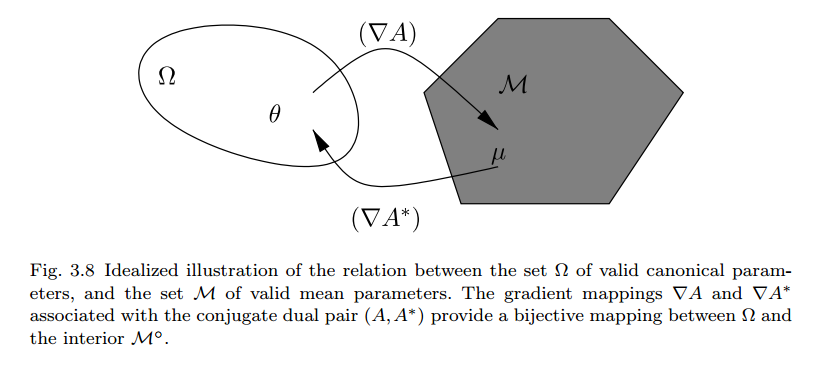
\includegraphics[scale = 0.45]{forward_backward_mapping.png}}
\end{minipage}
\caption{\footnotesize{\textbf{The forward and backward mapping between the cannoical parameter region to the marginal polytope.}}}
\label{fig: forward_backward_mapping}
\end{figure}


The convex \textbf{\emph{conjugate dual}} of log-partition function $A$ is defined as 
\begin{align}
A^{*}(\mb{\mu}) &:= \sup_{\mb{\eta} \in \Omega} \set{\inn{\mb{\mu}}{\mb{\eta}} - A(\mb{\eta})} \label{eqn: conjugate_dual_partition}
\end{align} Here $\mb{\mu} \in \bR^{d}$ is a fixed vector of so-called \textbf{dual variables} of the same dimension as $\mb{\eta}$. 

The conjugate dual function \eqref{eqn: conjugate_dual_partition} is the \textbf{negative} \textbf{entropy}. When $\mb{\mu} \in \cM^{\circ}$, then 
\begin{align*}
A^{*}(\mb{\mu})  &= \int \log q(\mb{x}; \mb{\eta}(\mb{\mu})) \, q(\mb{x}; \mb{\eta}(\mb{\mu})) \nu(d\mb{x})  := -H(q_{\mb{\eta}(\mb{\mu})}), 
\end{align*} where the $q$ is the exponential family \eqref{eqn: exp_fam} with canonical parameter $\mb{\eta}(\mb{\mu})$ and the moment matching conditions are met
\begin{align}
\E{\mb{\eta}(\mb{\mu})}{\mb{\phi}(X)} &= \mb{\mu} \label{eqn: dual_condition}
\end{align} This fact is essential in the use of \textbf{variational methods}: it guarantees that any optimization problem involving the dual function can be reduced to an optimization problem over $\cM$.

\begin{theorem}\label{theorem: dual_A} \citep{wainwright2008graphical}
\begin{enumerate}
\item For any $\mb{\mu} \in \cM^{\circ}$, denote by $\mb{\eta}(\mb{\mu})$ the unique canonical parameter satisfying the dual matching condition \eqref{eqn: dual_condition}. The conjugate dual function $A^{*}$ takes the form
\begin{align}
A^{*}(\mb{\mu}) &= \left\{\begin{array}{cc}
 -H(q_{\mb{\eta}(\mb{\mu})}) & \text{ if }\mb{\mu} \in \cM^{\circ}\\
+\infty & \text{ if }\mb{\mu} \not\in \overline{\cM}
\end{array} \right. \label{eqn: conjugate_dual_partition_neg_ent}
\end{align}
For any boundary point $\mb{\mu} \in  \partial \cM := \overline{\cM} \setminus \cM^{\circ}$ we have
\begin{align}
A^{*}(\mb{\mu}) &= \lim_{n\rightarrow \infty} A^{*}(\mb{\mu}_{n})
\end{align} taken over any sequence $\{\mb{\mu}_n\} \subset \cM^{\circ}$ converging to $\mu$.

\item In terms of this dual, the log-partition function has the \textbf{variational representation}
\begin{align}
A(\mb{\eta}) &=  \sup_{\mb{\mu} \in \cM}\set{ \inn{\mb{\eta}}{\mb{\mu}} - A^{*}(\mb{\mu})} \label{eqn: log_partition_variational_form}
\end{align}

\item For all $\mb{\eta} \in \Omega$, the supremum in Equation \eqref{eqn: log_partition_variational_form} is attained uniquely at the vector $\mb{\mu} \in \cM^{\circ}$ specified by the moment matching conditions
\begin{align}
\E{\mb{\eta}}{\mb{\phi}(X)} &= \int_{\cX^{m}} \mb{\phi}(\mb{x}) q(\mb{x};\mb{\eta})\nu(d\mb{x}) = \mb{\mu} \label{eqn: dual_condition}
\end{align} 
\end{enumerate}
\end{theorem}

The above theorm establishes the duality between log-partition function $A$ and negative entropy $A^{*}$. Note that $A^{*}$ is a function of mean parameter $\mb{\mu}$ not like usual entropy as function of distribution. Moreover, the value $-A^{*}(\mb{\mu})$ corresponds to the \textbf{optimal value} of maximum entropy optimization \eqref{eqn: max_ent}.  Thus \eqref{eqn: log_partition_variational_form} formulate the maximum entropy estimation problem in \eqref{eqn: max_ent}. Third, above theorem  also clarifies the precise nature of the \textbf{\emph{bijection}} between the \underline{sets $\Omega$ and $\cM^{\circ}$}, which holds for any minimal exponential family.  In particular, the gradient mapping $\grad{}{A}$ maps $\Omega$ in a one-to-one manner onto $\cM^{\circ}$, whereas the \textbf{\emph{inverse mapping}} from $\cM^{\circ}$ to $\Omega$ is given by the gradient $\grad{}{A^{*}}$ of the dual function. The mapping $\grad{}{A^{*}}: \cM^{\circ} \rightarrow \Omega$ is called \underline{\textbf{\emph{backward mapping}}}.  See Figure \ref{fig: forward_backward_mapping} for an idealized illustration of this \textbf{bijective} correspondence based on the gradient mappings $(\grad{}{A}, \grad{}{A^{*}})$.

With conjugate dual, we see that the \textbf{\emph{maximum likelihood estimation}} problem is essentially the \underline{\textbf{dual problem}} of the maximum entropy estimation \eqref{eqn: max_ent}.
\begin{align}
\max_{\mb{\eta}} &\; \frac{1}{N}\sum_{n=1}^{N}\log q_{\mb{\eta}}(X_{n}) \nonumber\\
\Rightarrow \max_{\mb{\eta}}&\, \inn{\bar{\mb{\mu}}}{\mb{\eta}} - A(\mb{\eta}) \label{eqn: mle}
\end{align} where $\bar{\mb{\mu}} = \hat{\mathds{E}}_{}[\mb{\phi}(X)] = \frac{1}{N}\sum_{n=1}^{N}\mb{\phi}(X_{n})$ fits the moment matching conditions.  \eqref{eqn: mle} is the right-hand side of the conjugate dual of log-partition function $A^{*}$ in \eqref{eqn: conjugate_dual_partition}. Thus we have one statistical interpretation of this variational problem \eqref{eqn: conjugate_dual_partition}: $A^{*}$ is the \textbf{optimal value of the rescaled log likelihood} \eqref{eqn: mle}. 

Also see that the gradient of log-likelihood function 
\begin{align}
\grad{\mb{\eta}}{\frac{1}{N}\sum_{n=1}^{N}\log q_{\mb{\eta}}(X_{n}) }&= \grad{\mb{\eta}}{\paren{\inn{\bar{\mb{\mu}}}{\mb{\eta}} - A(\mb{\eta}) }} \nonumber\\
&=  \hat{\mathds{E}}_{}[\mb{\phi}(X)] - \E{\mb{\eta}}{\mb{\phi}(X)} \label{eqn: grad_log_likelihood}\\
&=  \bar{\mb{\mu}} - \mb{\mu}  = \text{sample mean} - \text{model mean}  \nonumber
\end{align}

\subsection{Challenges in high dimensional setting}
\begin{figure}
\begin{minipage}[t]{1\linewidth}
  \centering
  \centerline{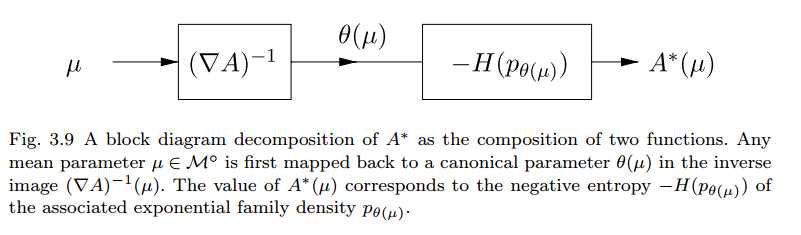
\includegraphics[scale = 0.45]{A_dual.png}}
\end{minipage}
\caption{\footnotesize{\textbf{The computation of $A^{*}$.}}}
\label{fig: A_dual}
\end{figure}
For general multivariate exponential families, there are two \textbf{primary challenges} associated with the \textbf{variational representation}:
\begin{enumerate}
\item In many cases, the constraint set $\cM$ of realizable mean parameters is extremely difficult to characterize in an \textbf{explicit} manner. Note that even in discrete cases, the number of constraints defining $\cM$ grows exponentially with respect to dimension of sample space $\cX^{m}$.

\item The negative entropy function $A^{*}$ is defined indirectly in a variational manner so that it too typically \textbf{lacks an explicit form}.
\end{enumerate}

To understand the complexity inherent in evaluating the dual value $A^{*}(\mb{\mu})$, note that Theorem 2.4 provides only an implicit characterization of $A^{*}$ as the \textbf{composition} of mappings: first, the \textbf{inverse mapping} $(\grad{}{A})^{-1}: \cM^{\circ} \rightarrow  \Omega$, in which $\mb{\mu}$ maps to $\mb{\eta}(\mb{\mu})$, corresponding to the \emph{exponential family member} with \textbf{mean parameters} $\mb{\mu}$; and second, the mapping from $\mb{\eta}(\mb{\mu})$ to the negative entropy $-H(q_{\mb{\eta}(\mb{\mu})})$ of the associated exponential family density. This decomposition of the value $A^{*}(\mb{\mu})$ is illustrated in Figure \ref{fig: A_dual}. Computing the inverse mapping $(\grad{}{A})^{-1}$ as well as entropy $-H$ are both challenging in high dimensional setting. These difficulties motivate the use of \textbf{approximations} to $\cM$ and $A^{*}$.

\subsection{Primal-dual formulation of KL divergence}
\begin{figure}
\begin{minipage}[t]{1\linewidth}
  \centering
  \centerline{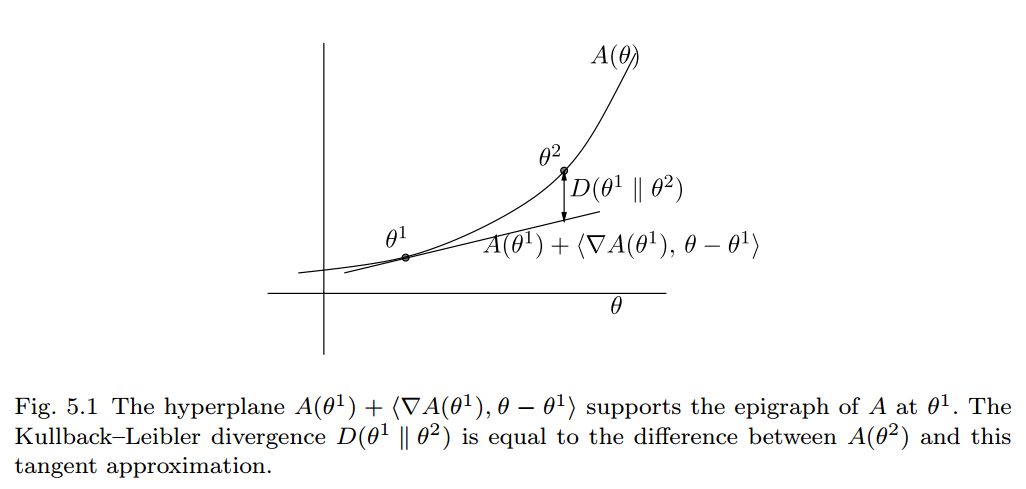
\includegraphics[scale = 0.4]{kl_divg_geo.png}}
\end{minipage}
\caption{\footnotesize{\textbf{The geometrical intepretation using primal $A$ and dual $A^{*}$}}}
\label{fig: kl_divg_geo}
\end{figure}

The conjugate duality between $A$ and $A^{*}$, as characterized in Theorem \eqref{theorem: dual_A}, leads to several alternative forms of the KL divergence for
\emph{exponential family members}.
\begin{align*}
\kl{q}{p} &:= \int_{\cX^{m}} q(x) \log\brac{\frac{q(x)}{p(x)}} \nu(dx)
\end{align*} Consider two canonical parameter vectors $\mb{\eta}_1, \mb{\eta}_2 \in \Omega$, we formulate the KL divergence between two distributions in exponential family
\begin{align}
\kl{p_{\mb{\eta}_1}}{p_{\mb{\eta}_2}} &\equiv  \kl{\mb{\eta}_1}{\mb{\eta}_2}\nonumber\\
&:= \E{\mb{\eta}_1}{A(\mb{\eta}_2) - A(\mb{\eta}_1)  -\inn{\mb{\phi}(X)}{\mb{\eta}_2 - \mb{\eta}_1} } \nonumber\\
&=  A(\mb{\eta}_2) - A(\mb{\eta}_1) -  \inn{\mb{\mu}_{1}}{\mb{\eta}_2 - \mb{\eta}_1}  \label{eqn: kl_primal}\\
&\equiv  A(\mb{\eta}_2) - A(\mb{\eta}_1) -  \inn{\grad{}{A}(\mb{\eta}_1)}{\mb{\eta}_2 - \mb{\eta}_1}  \nonumber
\end{align} where $\mb{\mu}_{1} = \E{\mb{\eta}_1}{\mb{\phi}(X)} = \grad{}{A}(\mb{\eta}_1)$ is the mean parameters for $p_{\mb{\eta}_1}$. This is the \textbf{\underline{\emph{primal form}} of the KL divergence} at $p_{\mb{\eta}_1}$. As illustrated in Figure \ref{fig: kl_divg_geo}, this form of the KL divergence can be
interpreted as the difference between $A(\mb{\eta}_2)$ and the \emph{hyperplane \textbf{tangent}} to $A$ at $\mb{\eta}_1$ with normal $\grad{}{A}(\mb{\eta}_1) = \mb{\mu}_{1}$. 

A second form of the KL divergence can be obtained by using the strong duality condition \eqref{eqn: log_partition_variational_form} for dually coupled parameters.
\begin{align}
 \kl{\mb{\eta}_1}{\mb{\eta}_2} \equiv  \kl{\mb{\mu}_1}{\mb{\eta}_2}&= A(\mb{\eta}_2) - A(\mb{\eta}_1) -  \inn{\mb{\mu}_{1}}{\mb{\eta}_2 - \mb{\eta}_1} \nonumber\\
&= A(\mb{\eta}_2) - \paren{\inn{\mb{\mu}}{\mb{\eta}_1} - A^{*}(\mb{\mu}_{1})} -  \inn{\mb{\mu}_{1}}{\mb{\eta}_2 - \mb{\eta}_1}  \nonumber\\
&= A(\mb{\eta}_2) + A^{*}(\mb{\mu}_1) - \inn{\mb{\mu}_{1}}{\mb{\eta}_2}  \label{eqn: kl_primal_dual}
\end{align} This is the \textbf{\emph{\underline{primal-dual mixed form}} of the KL divergence}.

Finally, we have the \textbf{\emph{\underline{dual form}} of KL divergence}: 
\begin{align}
 \kl{\mb{\mu}_1}{\mb{\mu}_2} &= A(\mb{\eta}_2) + A^{*}(\mb{\mu}_1) - \inn{\mb{\mu}_{1}}{\mb{\eta}_2}  \nonumber\\
 &= \inn{\mb{\mu}_2}{\mb{\eta}_2} - A^{*}(\mb{\mu}_{2}) + A^{*}(\mb{\mu}_1) - \inn{\mb{\mu}_{1}}{\mb{\eta}_2}  \nonumber\\
 &= A^{*}(\mb{\mu}_1) - A^{*}(\mb{\mu}_{2}) - \inn{\mb{\eta}_2}{\mb{\mu}_{1} - \mb{\mu}_{2}}  \label{eqn: kl_dual} \\
 &\equiv  A^{*}(\mb{\mu}_1) - A^{*}(\mb{\mu}_{2}) - \inn{\grad{}{A^{*}}(\mb{\mu}_{2})}{\mb{\mu}_{1} - \mb{\mu}_{2}} \nonumber
\end{align} The dual form is related to the \emph{Bregman divergence}, which induce the \textbf{projection operation}:
\begin{definition}
Let $F: \cX \rightarrow \bR$ be a \emph{continuously-differentiable}, \emph{\textbf{strictly convex}} function defined on a convex set $\cX$. The \textbf{\emph{Bregman divergence}} associated with $F$ for points $p,q \in \cX$ is the difference between the value of $F$ at point $p$ and the value of the \emph{first-order Taylor expansion} of F around point $q$ evaluated at point $p$:
\begin{align}
\divg{F}{p}{q} &= F(p) - F(q) - \inn{\grad{}{F}(q)}{p - q} \label{eqn: bregman_divg}
\end{align} we see that dual form $\kl{\mb{\mu}_1}{\mb{\mu}_2} = \divg{A^{*}}{\mb{\mu}_1}{\mb{\mu}_2}$, where $F = A^{*}$ is the negative entropy.
\end{definition}

\newpage
\bibliographystyle{plainnat}
\bibliography{book_reference.bib}
\end{document}